\documentclass[a4paper]{report}
\usepackage[utf8]{inputenc}	% translate UTF-8 into ASCII code for latex
\usepackage[T1]{fontenc}		% encodes non ASCII characters as single character and not a characte + accent mark
\usepackage[english]{babel}	% locales for laguages (here only English)
\usepackage{graphicx}		% images
\usepackage[margin=0.15\linewidth]{geometry}	% geometry package, set page margins
\usepackage{hyperref}	% references and metadata; contains nameref package for smart ref.
\usepackage{tabularx}	% tables
\usepackage{amsmath,amsfonts,mathtools}	% math tools
\usepackage{fontawesome}	% symbols (this is v4.7)
\usepackage{tikz,pgf,pgfplots}	% tikz packages, pgf plots package
\usepackage{caption}
% note that for system without Computer Modern, T1 is bitmap font, so in such case, use package  lmodern
%===================================================%
% Metadata settings
\hypersetup{	pdftitle={Zero model report},
			pdfauthor={Daniel \v{S}m\'{i}t},
			pdfsubject={Zero model for transport problem},
			pdfcreator={Daniel \v{S}m\'{i}t},
			pdfkeywords={O-D matrix, transportation, optimization, zero model},
			pdfdisplaydoctitle={true}}

%===================================================%
% Tikz styles
\usetikzlibrary{calc}			% coordinate calculation
\usetikzlibrary{arrows.meta, angles, quotes}	% arrowheads
\usetikzlibrary{intersections}
\usepgfplotslibrary{fillbetween}	% fill area between curves
\tikzset{location/.style={anchor=center, inner sep=4pt, font=\Large, draw=black,very thick, minimum width=4em, minimum height=4em,fill=blue!10!white}}%
\tikzset{tripline/.style={rounded corners=10pt,very thick, -{Latex[]}}}%
\tikzset{labelnode/.style={draw=none,font=\large,midway, above, outer sep=3pt}}%
\tikzset{smallabel/.style={draw=none, font=\Large, anchor=north west, outer sep=2pt}}%
\tikzset{graphlbl/.style={red, font=\large, above, sloped,midway}}%
\tikzset{dot/.style = {circle, fill, minimum size=#1,inner sep=0pt, outer sep=0pt}}%
\pgfplotsset{width=0.8\linewidth, height=0.6\linewidth}%


%===================================================%
% Commands and shortcuts
\renewcommand*\thesection{\arabic{section}}	% redefine section number to omit chapter number
\newcommand\trip{$A\rightarrow{}E$}		% shortcut for A->B

% Roman numeral macro
\makeatletter
\newcommand*{\rom}[1]{\expandafter\@slowromancap\romannumeral #1@}
\makeatother

% Declare floor function
\DeclarePairedDelimiter\floor{\lfloor}{\rfloor}
\DeclarePairedDelimiter\ceil{\lceil}{\rceil}
\DeclarePairedDelimiter{\nint}{\lfloor}{\rceil}
\DeclareMathOperator*{\argmax}{arg\,max}



\begin{document}

\section{Introduction}
The following basic 'zero model' serves as a proof-of-concept to demonstrate the basic idea and approach to the optimization of car fleet deployment within a specific feeding corridor zone $A$ at the time of peak hour. For this purpose we can use data of O-D matrix, $T_{AB}$ which gives number of trips between points $A$ and $B$ in one day. Based on those data, we can estimate $t_{AB}(t)$ as a number of traveling people per unit time from $A$ to $B$ at the time $t$ so that $\int\limits_{\text{day}} t_{AB}(t') dt' = T_{AB}$. 

Further, in this analysis, we will consider the situation during a morning (or evening) peak hour, when majority of people commute to work from the residential zone $A$ to a destination $B$. We assume that all of those taking the trip by mass public transport (MPT) make transfer to a backbone transport (e.g. light-rail or underground train) at the site $E$. We can describe the system as illustrated in \autoref{scheme} and defined in \autoref{tab:descriptors}.

\begin{figure}[ht]
\centering
	\begin{tikzpicture}
		\node[anchor=east, draw=black, thick, fill=red!05!white, minimum width=10em, minimum height=10em] (Azone) {};
		\node[smallabel, anchor=north west] (Apop) at (Azone.135) {\faUser\; $p_A$};
		\node[smallabel] (Aclock) at (Apop.south west) {\faHourglassHalf\; $c_s$,$d$};
		\node[smallabel] (Acrowd) at (Aclock.south west) {\faGroup\; $c_c$};
		\node[smallabel] (Awalk) at (Acrowd.south west) {\faStreetView\; $r$};
		\node[location,anchor=east](A) at (Azone.east) {A};
		\node[location](E) at ($(A.east)+(15em,0)$) {E};
		\node[location](B1) at ($(E.east)+(10em,5em)$) {B1};
		\node[location](B2) at ($(E.east)+(10em,0em)$) {B2};
		\node[location](B3) at ($(E.east)+(10em,-5em)$) {B3};
		\draw[tripline](A)--(E) node[labelnode] {$p_A(t)=\sum\limits_{\forall B} t_{AB}(t)$} node[labelnode, below]{$\tau,m,n$};
		\coordinate(center) at ($(E)!0.5!(B2)$);
		\draw[tripline](E.20) --+ (3em,0) |- (B1.west);
		\draw[tripline](E.-20) --+ (3em,0) |- (B3.west);
		\draw[tripline](E.east) -- (B2.west);	
	\end{tikzpicture}
	\caption{Scheme of transport along the \trip{} feeding corridor}
	\label{scheme}
\end{figure}

We define the following symbols, in general, all of them would be time-dependent:
\begin{table}[ht]
	\begin{tabular}{l p{0.3\textwidth} p{0.6\textwidth}}
	symbol		& 	name							& note\\\hline
	$t_{AB}(t)$	& 	origin-destination (o-d) flow				& Origin-destination flow of people per unit time from $A \rightarrow B$\\
	$p_A(t)$		&	susceptible population flow			& $p_A(t)=\sum\limits_{\forall B} t_{AB}(t)$, prospect clients going \trip{} per unit time\\
	$p_c(t)$		&	critical population flow				& critical level, if $p_A>p_c$, people start to take taxi\\
	$\Pi(t)$		& 	taxi rate							& probability of a single agent to take a taxi \\
	$q(t)$		& 	customer flow						& number of customers transported per unit time\\
	$c(t)$		&	personal cost						& perceived monetary cost of taking MPT of an agent\\
	$a(t)$		& 	(deployed) car capacity				& number of people possibly transported per unit time\\
	$m(t)$		&	taxi price/fare						& price of a taxi ride per person $A\rightarrow E$\\
	$\tau(t)$		& 	taxi roundtrip time					& mean time for taxi to drive $A\rightarrow E\rightarrow A$\\
	$s(t)$		& 	driver salary						& driver pay per unit time\\
	$n(t)$		&	deployed cars						& number of cars deployed for the trip $A\rightarrow E$\\
	$d(t)$		&	waiting time						& mean waiting time for MTP\\
	$r$			&	walking time						& mean walking time to reach MTP\\
	$c_s$		& 	time cost 							& mean monetary value of personal time ($\approx$ hourly wage)\\
	$c_c$		&	crowding cost						& mean monetary coefficient of crowd discomfort in MPT per person\\
	$c_M$		&	car capacity						& maximum number of passengers per taxi\\
	$i(t)$			&	income/return rate 					& money earned (or lost) per unit time; net income\\
	$i^{+}(t)$		&	collected fare/revenue rate			& money collected per unit time; brute income\\
	$i^{-}(t)$		& 	operation costs						& money spent on operations per unit time\\
\hline
	\end{tabular}
\caption{Definition of the descriptive parameters}%
\label{tab:descriptors}%
\end{table}%

Note, that most of the symbols are defined as rates, i.e. per unit time. Total quantity per interval $T$ is then calculated by integrating over time, e.g. $$Q=\int_T q(t')dt'$$ would be total number of clients $Q$ served during the interval $T$. For time independent rates integration reduces to simple multiplication, e.g. $q(t)=q: Q=q\cdot T$. %

\section{Simplification}
\label{sec:simple}
For sake of simplicity, we will treat only the morning peak time. We assume that during the morning peak period, the descriptors in \autoref{tab:descriptors} remain roughly constant (i.e. $p_A(t)=p_A, \Pi(t)=\Pi, s(t)=s$, etc.). We make the following simplifying assumptions:
\begin{enumerate}
	\item we consider only two available modes of transport, MPT and taxi
	\item people along the feeding corridor take transport from the given location $A$ to the MPT exchange hub $E$, the population flow originating in $A$ is $p_A$
	\item the susceptible population flow $p_A$ is much larger than the number of people in taxis or the taxi capacity ($p_A\gg a \geq q$) and so the amount of people taking taxi have no feedback on the system, or on the personal perceived cost of entering agents
	\item return trips of taxi $E\rightarrow{} A$ are without clients, the travel time difference between a taxi and MPT is ignored
	\item taxi drivers are paid flat rate per time unit $s$, and a taxi passenger pays a flat rate per seat $m$, independent of car occupancy
	\item all taxi trips \trip{} are of equal length, time ($\frac{\tau}{2}$), and fare ($m$), cost of MPT is considered negligible
	\item all $n$ deployed taxi cars are effectively identical, with maximum capacity per car $c_M$
	\item all traveling agents are identical (represented by constant mean values) and have perfect knowledge of the system (e.g. current descriptors), their MPT accessibility ($d$, $r$) is identical 
	\item agents are perfectly rational, they obey the cost function $c$.
\end{enumerate}%


\section{Cost function}
We define the function of perceived monetary costs of an agent stemming from the use of MPT. 
\begin{equation}
	c=\underbrace{c_s (d+r)}_{\text{MPT accessibility}}  + \underbrace{c_c p_A d}_{\text{crowding}}
	\label{eq:costfunction}
\end{equation}
The first term represents the perceived cost in terms of time lost walking ($r$) and waiting ($d$), converted to monetary cost by the factor $c_s$, which can be estimated as an hourly wage of an agent. The second term refers to the crowding (and discomfort) effect in the MPT, $p_A\,d$ is a mean occupancy of a bus dispatch, weighted by a factor $c_c$, persons sensitivity to discomfort.%

While many other factors play role, like tiredness, time of the day, weather, pedestrian infrastructure, MPT quality, reserved lanes for MPT, etc., we will neglect these in this analysis. Obviously, the variables that constitute the cost function would themselves be functions of time in a more general case. Note that the way the cost function is defined in \autoref{eq:costfunction}, it is constant for a given situation, and depends on the parameters of MPT ($d$, $r$) and demographics ($p_A$, $c_c$, $c_s$) of the zone $A$.%

\section{Personal choice and passenger flow}
In the simplest choice model, there is a threshold effect for the agent to choose alternative transportation mode---taxi in our case. This occurs when the perceived cost of MPT is higher that the taxi cost, $c>m$. This implies existence of a critical population flow $p_c(m)$ as a function of fare $m$ such, that the population in excess to this critical population flow $p_A>p_c$ opts for a taxi ride. That is, the probability of an entering agent to opt for a taxi is given as
\begin{equation}
\Pi=	\begin{cases}
		1: c(p_A)>m\\
		0: \text{otherwise}
	\end{cases}
\label{taxifreq}
\end{equation}
The critical population flow is given as 
\begin{align}
	c(p_A{=}p_c)&=m\nonumber\\
	m&=c_c p_c d + c_s(d+r)\nonumber\\
	p_c&= \frac{m-c_s(d+r)}{c_c d}\nonumber\\
	p_c(m)&=\underbrace{\frac{m}{c_c d}}_{\text{taxi cost}} - \underbrace{\frac{c_s(d+r)}{c_c d}}_{\text{MPT time cost}} \;\; |p_c\in \mathbb{R^{+}}\label{eq:criticalpopulation}
\end{align}%
Where the first term represents the demotivation effect of the taxi fare. The second term is the incentive of poor MPT accessibility---discomfort associated with reaching the MPT station. The critical flow $p_c$ is modulated by the crowding effect; high sensitivity to crowds and infrequent MPT decrease the critical flow threshold and represent a discomfort associated with traveling by MPT.%

The number of people taking a taxi per unit time, the passenger flow, is given as
\begin{align}
	q(m)&=\Pi(m) \cdot(p_A-p_c(m))\\ \label{eq:passangerflow}
	q(m)&=\begin{cases}
			\min\left(-\frac{m}{c_c d}+p_A+\frac{c_s(d+r)}{c_c d},p_A\right)\;\;\ |\text{if } c>m \nonumber\\
			0\;\; |\text{otherwise}
		\end{cases}			
\end{align}
We can see, that passenger flow $q(m)$ decreases with growing fare $m$ up to a halt at $c<m$.
The passenger flow in the taxis is limited by the taxi fleet capacity per unit time
\begin{equation}
	a(n)=\frac{c_M\, n}{\tau}.	\label{eq:taxicapacity}
\end{equation}
which depends only the number of cars $n$ (other factors are predetermined).%


\def\pd{p_A^{\dagger}}
\section{Income analysis}
The return rate is given as follows
\begin{equation}
	i(m,n) =\underbrace{\min{} (q(m),a(n)) \cdot m}_{\text{collected fare}; i^+} - \underbrace{s\cdot n}_{\text{operation cost}; i^-} \label{eq:revenuerate}
\end{equation}
under the predetermined zone parameters (e.g. $p_A, d, r$), operator can adjust two parameters: the fare $m$ which determines the passenger flow $q(m)$, and the deployed capacity $a(n)$ by sending $n$ cars. We denote the collected revenue per unit time $i^{+}$. The cost of operation per unit time, denoted $i^{-}$, is a sum of flat rates $s$ of all the drivers. Total return rate is $i=i^{+}-i^{-}$. This can be illustrated by the following (qualitative) \autoref{gr:incomegraph}

\begin{figure}[h]
\centering
	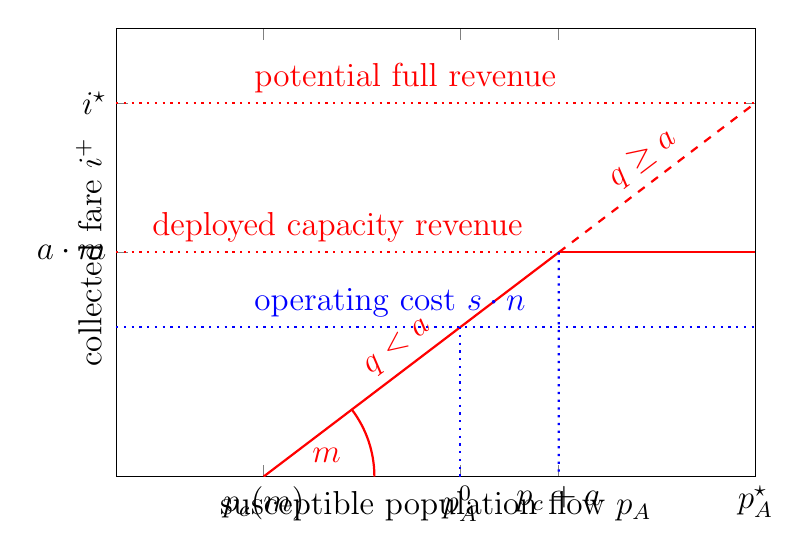
\begin{tikzpicture}
	\pgfplotsset{width=0.8\linewidth, height=0.6\linewidth}
	
	\begin{axis}[name=thisgraph,
		x label style={at={(axis description cs:0.5,0)}, anchor=north, outer sep=2pt},
		y label style={at={(axis description cs:0,0.5)}, anchor=south, outer sep=2pt},
		xmin=15,xmax=80, ymin=0, ymax=60,
		xlabel={\large susceptible population flow $p_A$}, ylabel={\large collected fare $i^{+}$},
		ticklabel style={font=\large},
		ytick = {30, 50}, xtick = {30, 50, 60, 80},
		xticklabels={ {$p_c(m)$}, {$p_A^{0}$}, {$p_c+a$}, {$p_A^{\star}$} }, yticklabels={ {$a\cdot m$}, {$i^{\star}$} } 
		]

		\addplot [domain=30:60,draw=red, thick, name path=customer]{x-30} node[graphlbl] {$q<a$};
		\addplot [domain=60:80, draw=red, thick, dashed] {x-30} node[graphlbl] {$q\geq a$} ;
		\addplot [domain=60:80, draw=red, thick] {30};
		\addplot [domain=15:60, draw=red, thick, dotted, name path=capacity] {30} node[graphlbl] {deployed capacity revenue};
		\addplot [domain=15:80, draw=red, thick, dotted] {50} node[graphlbl,pos=0.2, anchor=south west]{potential full revenue};
		\addplot [domain=15:80, draw=blue, thick, dotted, name path=operation] {20} node[graphlbl, blue,pos=0.2, anchor=south west] {operating cost $s\cdot n$};
		\coordinate (xline) at (axis cs: 60,0){};
		\coordinate(trendline) at (axis cs: 60,30);
		\coordinate(critpop) at (axis cs: 30,0);
		\pic [draw=red, "$m$", angle radius=4em, angle eccentricity=0.6, thick, text=red, font=\large] {angle = xline--critpop--trendline};
		\draw[blue, thick, dotted, name intersections={of=customer and operation}] (intersection-1) -- (axis cs: 50, \pgfkeysvalueof{/pgfplots/ymin});
		\draw[blue, thick, dotted, name intersections={of=customer and capacity}] (intersection-1) -- (axis cs: 60, \pgfkeysvalueof{/pgfplots/ymin});
	\end{axis}%

	\end{tikzpicture}
\caption{Illustration of the return rate $i^+$ dependence (red full line) on the susceptible population flow $p_A$. For optimally adjusted $m$ and $n$, the full revenue rate $i^\star$ is reached, if all population flow $p_A^\star$ is served.}
\label{gr:incomegraph}
\end{figure}%

In the \autoref{gr:incomegraph}, $a(n)\cdot m$ is the maximum revenue under the deployed fleet capacity, $i^\star$ is the maximal potential revenue and $p_A^\star$ is the corresponding susceptible population flow. $p_A^0$ is the value where the operation breaks even, i.e. $i(p_A^0)=0$. The blue dotted line represent the operation cost of the deployed fleet.%

Note that the collected fare $i^+$ (the full red line) depends on $m$. The fare $m$ adjusts the participation threshold $p_c$ (decreasing $m$ motivates people to move into taxis and adjusts the position of $p_c$ on the abscissa to the left) and the slope of the revenue line. $p_c$ does not depend on $n$, but is determined by the fixed characteristics of the residential area (see \autoref{eq:criticalpopulation} for details).%

As we can see in \autoref{gr:incomegraph}, there are four distinct zones depending on the susceptible population flow $p_A$:
\begin{itemize}
	\item zone \rom{1}: $p_A \in (0,p_c)$, there is no traffic, people prefer to take MPT. $i=-s\cdot n<0$
	\item zone \rom{2}: $p_A \in (p_c, p_A^0)$, clients opt to take taxi, there are sufficient capacities to cater all the clients, operation is at loss. $i=q\cdot m -s\cdot n<0$.
	\item zone \rom{3}: $p_A \in (p_A^0, p_c+a)$,  the same as \rom{2}, but operation is at surplus. $i=q\cdot m-s\cdot n>0$
	\item zone \rom{4}: $p\in (p_c+a, p_A^{\star})$, transportation of clients is throttled by the insufficient deployed car capacity. $i=a\cdot m-s\cdot n>0$.
\end{itemize}

Note that in the \autoref{gr:incomegraph}, we assume the operating cost is below the collected revenue ($i^+>i^-$) if the deployed fleet is fully occupied; in other words, adding another car, if it is full exploited, increases the return rate $i$; or, the cars are not subsidized. However, this does not need to be the case in general, and depends on the company adjustment of $s$ and $m$. To avoid loss on fully exploited fleet (passenger flow exceeds the deployed capacity), the condition is
\begin{align*}
	a\cdot m &\geq s\cdot n\\
	\frac{c_M\, n}{\tau}m &\geq s\cdot n\\
	\frac{c_M}{\tau}m &\geq s
\end{align*}
which means
\begin{equation}
	m\geq\frac{s\tau}{c_M}	\label{eq:feasiblerate}
\end{equation}
to assure feasibility of fully engaged cars.

We can now analyze the particular break points and optimal strategies of selection of parameters $m$ and $n$.%

\def\md{m^{\dagger}}
\def\cd{c^{\dagger}}
\subsection{Break even point}
\label{ss:breakeven}
Assume we are running on a feasible choice of parameter $m$ (\autoref{eq:feasiblerate}), and that the fleet capacity was not exceeded, $q\leq a$ (see \autoref{gr:ridepricegraph}). In such case, the collected revenue is given as $i^{+}=q\cdot m$. The costs associated are $i^-=s\cdot n$. If \autoref{eq:feasiblerate} holds, then for fixed predetermined choice of $m$ and $n$, there exist susceptible population flow $p_A^0$, and surpassing this flow yields positive revenue rate $i(p_A\geq p_A^0)\geq 0$, i.e. we break even, as noted in \autoref{gr:incomegraph}. However, we can also invert the problem: that is, what parameter $\md$ do we need to set for a predetermined population flow $\pd$\footnote{We use dagger ($\dagger$) to denote, that the variable is fixed to a particular value in this context. I.e. $\pd$ is a predetermined population flow, and $\md$ is a fixed operations parameter to meet a specific goal.}, to break even.
\begin{align*}
	i^{+}=q(\pd,\md)\cdot \md&=s \cdot n\\
		(\pd - p_c)\cdot \md&=s\cdot n\;\;| \text{using \autoref{eq:criticalpopulation}}\\
		\left[\pd -\frac{\md}{c_c d}+\frac{c_s}{c_c d} (d+r)\right]\md&=s\cdot n\\
		(\md)^2-\md\underbrace{(\pd c_cd +c_s(d+r))}_{\equiv \cd} 		&=-snc_cd\\
		(\md)^2-\md \cd + snc_cd &=0\\
		\md_{\text{<,>}}&=\frac{1}{2}\left[\cd\pm\sqrt{(\cd)^2-4sc_cdn}\right]
\end{align*}

This result tells us, that for a given $n$ (costs depend on $n$) and a fixed $\pd$, there are two pricing limits we can choose to break even. One such option involves fewer customers and higher price $\md_>$, the other would be pricing which attracts more customers at lower fare (which has a marketing benefit) at

\begin{equation}
	\md_{\text{<}}=\frac{1}{2}\left[\cd-\sqrt{(\cd)^2-4sc_cdn}\right]	\label{eq:breakeven}
\end{equation}

Actually, any price in the range $\md \in (\md_<,\md_>)$ yields feasible operation, which is visible, if we plot the graph of return rate as a function of $i(m)$, for $n: q(\md)\leq a(n)$, as shows \autoref{gr:ridepricegraph}. From the graph, we can also read, that for non-throttled situation, the maximum return rate choice of ride price is half of the perceived MPT cost, $m=\frac{\cd}{2}$.%

A technical question remains: the determinant in the \autoref{eq:breakeven} must remain positive. We can make order of magnitude realistic estimates of the parameters (with exception of crowd intolerance $c_c$, which is extremely subjective). For determinant to be positive, it is sufficient, if 
\begin{align*}
	[p_Ac_s(d+r)]c_cd&>4snc_cd\\
	p_Ac_s(d+r)&>4sn\;\;|s\sim c_s\\
	p_A(d+r)&>4n
\end{align*}
And considering that the total number of people leaving by MTP each turn is larger than the number of deployed cars ($p_A\gg a$, see \autoref{sec:simple}), and the other terms of $(\cd)^2$ expansion are always positive, we see that the determinant remains positive, and the solution with feasibility zone is guaranteed.

\begin{figure}[h]
\centering
	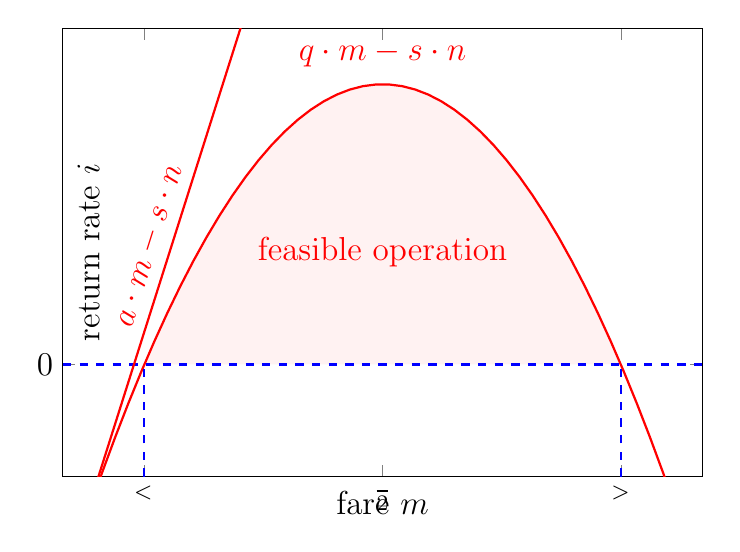
\begin{tikzpicture}
	\pgfplotsset{width=0.8\linewidth, height=0.6\linewidth}
	
	\begin{axis}[
		x label style={at={(axis description cs:0.5,0)}, anchor=north, outer sep=2pt},
		y label style={at={(axis description cs:0,0.5)}, anchor=north, outer sep=2pt},
		xmin=0,xmax=60, ymin=-200, ymax=600,
		xlabel={\large fare $m$}, ylabel={\large return rate $i$},
		ticklabel style={font=\large},
		ytick = {0}, xtick = { 7.6, 30, 52.4, 60},
		xticklabels={ {$\md_<$}, {$\frac{\cd}{2}$}, {$\md_>$}, {$\cd$} }, yticklabels={ 0} 
		]
soft clip={domain=0:1},
		\addplot [name path=income, domain=0:60, draw=red, thick, samples=50] { -(x-30)^2 + 500} node[graphlbl, outer sep=3pt] {$q \cdot m - s\cdot n$};
		\addplot [domain=0:60, draw=blue, thick, dashed] {0};
		\draw[blue, thick ,dashed] (axis cs: 7.6,-200) -- (axis cs: 7.6,0);
		\draw[blue, thick ,dashed] (axis cs: 52.4,-200) -- (axis cs: 52.4,0);
		\path[name path=zero] (axis cs: 0,0) -- (axis cs: 60, 0);
		\addplot [ thick, color=blue, fill=red, fill opacity=0.05] fill between[of=income and zero,soft clip={domain=7.6:52.4},];
		\node[font=\large, text=red] at (axis cs: 30, 200) {feasible operation};
		\addplot[red, thick, domain=0:20] {60*x-400} node [graphlbl] {$a\cdot m - s\cdot n$};
	\end{axis}

	\end{tikzpicture}
\caption{Illustration of the return rate dependence on the fare $m$ for a passenger flow $q(m)$ (parabola) and potential revenue at fleet capacity (line). Note that the return rate (for a sufficient but fixed capacity $n$ catering the passenger flow, $a(n)\geq q$) peaks at $m=\frac{\cd}{2}$. It drops to the the full operation loss for free rides ($i(0)=-s\cdot n$) and prices above client cost function ($i(m>\cd)=-s\cdot n$).}
\label{gr:ridepricegraph}
\end{figure}

The analysis of the break-even points is meaningful for adaptive pricing. It shows the boundaries of feasible operations and as such gives predictable space for special fare discount or benefits for the drivers.

\newpage
\def\ms{m^{\star}}
\def\ns{n^\star}
\def\ccd{\frac{c_Mc_cd}{\tau}}
\subsection{Maximal return rate}
\label{ss:maxretrate}
The last aspect of the model is maximizing the return rate $i(m,n)$. In the following sections, we assume a situation with no planned loss, as demanded by \autoref{eq:feasiblerate}, i.e. fully exploited car covers its operation costs. In the following, we will also assume a fixed susceptible population flow $\pd$, which means a fixed cost function $\cd$ (\autoref{eq:costfunction}). %

We formally analyze the return rate maximum ($i^\star$) without capacity constrains, we consider parameter $n$ chosen (and fixed) in such way, that $q(m)\leq a(n), \forall m$, that is, the capacity of the fleet of $n$ cars can serve all the potential customers. This is represented in \autoref{gr:ridepricegraph} by the parabola being smaller than the line for all relevant $m$. Now, we want to maximize the collected fare $i^+$ (operation costs $i^-(n)$ are given and fixed by the choice of $n$) by selecting the maximizing $\ms$\protect\footnote{We use the star symbol $\star$ to denote the parameter value, which was chosen and fixed to optimize for maximum return rate.}.
In absence of a capacity constraint, $\ms$ maximizes the return rates for a given $\pd$ and $n$.
\begin{align}
	m\overbrace{\left[\pd - \frac{m}{c_cd}+\frac{c_s}{c_cd}(d+r)\right]}^{=q\leq a}&=i^{+}\nonumber\\
	\frac{\partial i^{+}}{\partial m}=\left[\pd+\frac{c_s}{c_cd}(d+r)\right] - 2\frac{m}{c_cd}&=0\nonumber\\
	\ms=\frac{1}{2}\left[\pd c_cd+c_s(d+r)\right]&=\frac{\cd}{2}\;\;|\text{as shown in \autoref{gr:ridepricegraph}}\label{eq:maxreturngeneral}
\end{align}

\newcommand\msn[1]{$m_{#1}^{\star}$}
In a case more general than presented in \autoref{gr:ridepricegraph}, the total revenue rate corresponds to the transported passenger flow $q(m)$ under the fleet capacity constraint $a(n)$, and is given by $i^+=\min(q(m),a(n))\cdot m$ (see \autoref{eq:revenuerate} and illustrated in \autoref{gr:revenue}). The operational cost $i^-=s\cdot n$ is constant for a given fleet size $n_i$, whether we fully use the capacity $a(n_i)$ or not. We maximize the revenue rate $i$, if we set the relationship between $m$ and $n$ to fully exploit the available capacity under the given fleet size $n_i$ (illustrated in \autoref{gr:revenue}), that is, under the constraint $a(n_i)=q(\ms_i)$, the relationship yields
\begin{align}
	q(\ms_i)&= a(n_i)\nonumber\\
	\underbrace{\left[\pd - \frac{\ms_i}{c_cd}+\frac{c_s}{c_cd}(d+r)\right]}_{\text{total transported flow}}&=\underbrace{\frac{c_M\cdot n_i}{\tau}}_{\text{fleet capacity}} \nonumber\\
	 \ms_i&=\cd - \frac{c_Mc_cd}{\tau} n_i\label{eq:mnrelation}\;\;|\text{analogically to \autoref{ss:breakeven}}
\end{align}
Note that \autoref{eq:mnrelation} is met only by a limited set of tuples $(n_i,\ms_{i})$, where $n_i\in\mathbb{N}$ (because we only have integer cars). In other words, for each fleet size $n_i$, there is exactly one pricing model $\ms_i$ that yields the maximum return rate $i^\star_i$. Say we have 15 cars at hand, then there exist 15 distinct corresponding prices to optimize the revenue rate for each deployed fleet size (given by \autoref{eq:mnrelation}).%

Looking on the \autoref{eq:maxreturngeneral} and \autoref{eq:mnrelation} and looking on the \autoref{gr:revenue}, we note that the value of the optimal fare peaks at $\ms=\frac{\cd}{2}$, growing capacity beyond this point does not improve the revenue rate $i^+$ (but increases the costs $i^-$). We can write the optimal $\ms$ in two equivalent forms.%

\begin{align}
	\ms_i&=\argmax\limits_{m\in(\frac{\cd}{2},\cd); n=n_i} \{\min(a(n),q(m))\} \nonumber\\
	\ms_i&=\max\left(\frac{\cd}{2},\cd-\frac{c_Mc_cd}{\tau}n_i\right) \label{eq:mscomplete}
\end{align}

Under given circumstances of a market zone $A$ (i.e. $\pd, r, d, c_c$ etc.), we can select both $\ms$ and $\ns$ optimally, i.e. we can calculate the optimal fleet size $\ns$ and the corresponding optimal pricing $\ms$ for the given targeted zone $A$ to guarantee maximal income rate $i$. We can take two approaches to solve this problem. First, we can make a real number estimate of the globally optimal tuple $(\ns,\ms)\in \mathbb{R}$ using optimization method with Lagrange multipliers and then find the nearest optimal integer solution $\ns\in\mathbb{N}$. Second, we can look into the discrete differences of revenue rate as the fleet size is incremented. We will present both approaches in the following two sections.%

\begin{figure}[ht]
\centering

\tikzset{capacity/.style={domain=0:60, draw=red, thick}}
	\begin{tikzpicture}
	
	\begin{axis}[samples=50,
		x label style={at={(axis description cs:0.5,0)}, anchor=north, outer sep=2pt},
		y label style={at={(axis description cs:0,0.5)}, anchor=north, outer sep=2pt},
		xmin=0, xmax=60, ymin=-450, ymax=600,
		ylabel={\large revenue rate $i^+$}, xlabel={\large fare $m$},
		ticklabel style={font=\large},
		ymajorticks=false,
		xtick = { 0 , 30, 35, 40, 45, 50, 55, 60},
		xticklabels={ {0}, {$\frac{\cd}{2}$}, {\msn{5}}, {\msn{4}},{\msn{3}},{\msn{2}},{\msn{1}},{$\cd$} }, yticklabels={}
		]

		\path[name path=zero] (axis cs: 0,-400) -- (axis cs: 60,-400);
		\addplot [name path=served, domain=0:60, draw=red, thick] { -(x-30)^2 + 500};	
		\addplot [blue, dotted, thick, domain=0:60] {-400}; 	
		
		\pgfplotsinvokeforeach{1,2,3,4,5}
			{\edef\n{#1}
			{\edef\temp{\noexpand\addplot [name path=cap#1, capacity] { \n*5*x -400} node[graphlbl, sloped=false]{$n_\n$};}\temp}			
			\draw[dotted, thick, blue, name intersections={of=served and cap#1, by={inter1,inter2}}] (inter2) -- (inter2 |- 0,\pgfkeysvalueof{/pgfplots/ymin});
			}

		
		\addplot [ thick, color=blue, fill=red, fill opacity=0.05] fill between[of=served and zero,soft clip={domain=55:60},];
		\addplot [ thick, color=blue, fill=red, fill opacity=0.05] fill between[of=cap1 and zero,soft clip={domain=0:55},];
		\node[font=\large, text=red, anchor=south] at (axis cs: 40, -350) {potential revenue under $n_1$};
		
	\end{axis}
	\end{tikzpicture}
	\caption[revenue rate parabola]{The parabola represents the collected revenue rate curve for a given fare without any constraint of deployed fleet capacity. The lines labeled $n_i$ represent the revenue rates upper limits given by the fleet capacity $a(n_i)$. Points labeled \msn{i} label the optimal fare for the given fleet size $n_i$, i.e. \ensuremath{\ms_i=\argmax\limits_{\substack{ m\in(\frac{\cd}{2},\cd) \\ {n=n_i} } } \{\min(a(n_i),q(m))\}}. Note that the \msn{i} are equidistant.}
	\label{gr:revenue}
\end{figure}

\newpage
\subsubsection{Lagrange multiplier optimization}
We will find the optimal choice of pricing $\ms$ and fleet size $\ns$ for the revenue rate function (see \autoref{eq:revenuerate}) in the following non-throttled form (represented by the mesh in \autoref{gr:lagrangeproblem})
\begin{equation}
	i(m,n)=-\frac{m^2}{c_cd}+\frac{\cd}{c_cd}m-s\cdot n \label{eq:revenueratefree}
\end{equation}
under the the fleet capacity constraint with optimal pricing (see $m-n$ relation in \autoref{eq:mscomplete}, represented by the red constraining solid line in \autoref{gr:lagrangeproblem})
\begin{equation}
	g(m,n)=m - \max\left(\frac{\cd}{2},\cd-\frac{c_Mc_cd}{\tau}n\right)=0 \label{eq:lagrangeconst}
\end{equation}
For a given susceptible population flow $\pd$, there is a (real approximation of the) threshold fleet size $n_T\in \mathbb{R}$ (see \autoref{gr:lagrangeproblem}). After such threshold, adding more cars $n_k>n_T$ does not increase the maximal return rate, $\max(i(n_k)) < \max(i(n_T))$, and the pricing $\ms=\frac{\cd}{2}$ maximizes the revenue rate, $\argmax\limits_{m} i(m,n_k)=\frac{\cd}{2}$. The threshold is given as
\begin{align}
	\frac{\cd}{2}&=\cd-\ccd n_T \nonumber\\
	n_T&=\frac{\cd}{2}\frac{\tau}{c_Mc_cd} \label{eq:threshn}
\end{align}

\begin{table}[h!]
	\centering
	\begin{tabular}{p{0.45\textwidth}| p{0.45\textwidth}}
		$n < n_T$					& $n \geq n_T$ \\
		$m = \cd - \ccd n$			& $m = \frac{\cd}{2}$ \\
		$g(m,n)= m - \cd + \ccd n = 0$	& $g(m,n) = m - \frac{\cd}{2} = 0$\\ 
	\end{tabular}
	\caption{Two domains for optimization, depending on fleet size threshold $n_T$.}
	\label{tab:twolagrange}
\end{table}

We split our calculation into two domains, for $n<n_T$ and $n\geq n_T$ as sketched in \autoref{tab:twolagrange}.

For each of the two domains in \autoref{tab:twolagrange}, we solve the system
\begin{align*}
	\nabla_{m,n} \left[i(m,n)-\lambda g(m,n)\right]&=0\\
	g(m,n)&=0
\end{align*}
applying the technique of Lagrange multipliers, where $\lambda$ is a Lagrange multiplier.

\begin{figure}[ht!]
\centering
\pgfplotsset{width=0.95\linewidth, height=0.7\linewidth, compat=1.15}
	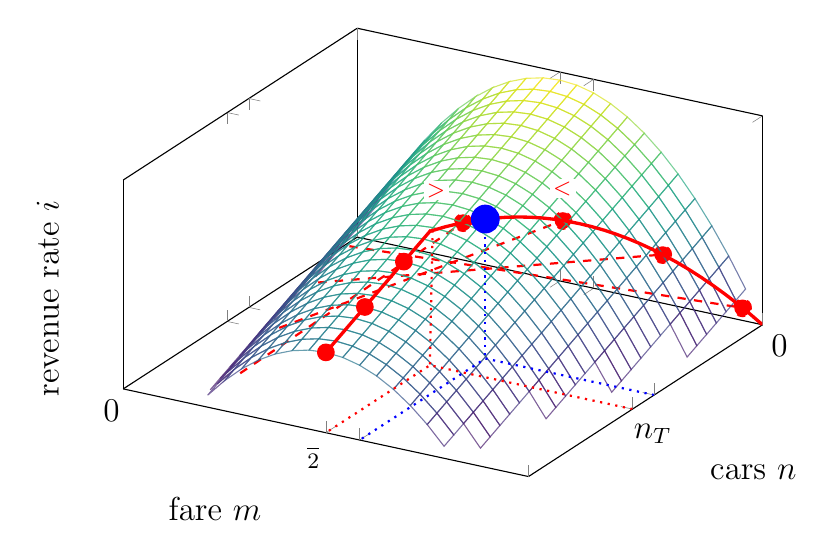
\begin{tikzpicture}
		\begin{axis}[view={120}{40},
				domain=0:30, domain y=0:100,
				zmin=0, zmax=2600, xmin=0, xmax=30, ymin=0, ymax=100,
				x label style={at={(axis cs: 15, 100 ,0)}, anchor=north west, outer sep=2em},
				y label style={at={(axis cs: 30, 50, 0)}, anchor=north east, outer sep=2em},
				z label style={outer sep=2em},
				ylabel={\large fare $m$}, xlabel={\large cars $n$}, zlabel={\large revenue rate $i$},
				ticklabel style={font=\large}, zmajorticks=false, %ymajorticks=false,
				xtick = { 0, 13.8888, 16.6666 }, ytick = {0, 50, 58.3333, 100}, 
				xticklabels={ 0, {$\ns$}, {$n_T$} }, yticklabels={0, $\frac{\cd}{2}$, $\ms$, $\cd$}
				]

			\pgfplotsinvokeforeach{1,5,10,15}
			{\edef\n{#1}
			\edef\nodename{node#1}
%			\pgfmathsetmacro{\limitA}{50-sqrt(2500-50*\n)}
			\pgfmathsetmacro{\intercept}{50*\n}
			\pgfmathsetmacro{\limitB}{100-3*\n}
			\pgfmathsetmacro{\slope}{(-9*\n*\n+250*\n+\intercept)/(100-3*\n)}
			{\edef\temp{\noexpand\addplot3 [thick, dashed, red, domain y=0:\limitB] ( {\n}, {y}, {\slope*y-\intercept} ) node (\nodename) [dot=6pt,draw=red,pos=1]{};}\temp}
			}
		      	\addplot3 [mesh, colormap/viridis, opacity=0.7,restrict z to domain=0:2500]{-(y-50)^2+2500-50*x};
			\addplot3 [very thick, red, restrict y to domain=50:100,samples=50, shorten >=-0.29ex] ( {x}, {100-3*x}, {-9*x^2+250*x} ) coordinate (ntnode);
			\addplot3 [very thick, red, restrict x to domain=16.4:30,samples=30] ( {x}, {50}, {2500-50*x} );
			\addplot3 [only marks, mark size=3pt, draw=red, fill=red] coordinates { (20, 50, 1500)  (25, 50, 1250)  (30, 50, 1000) };
			\addplot3 [only marks, mark size=5pt, draw=blue, fill=blue] coordinates { (13.88888, 58.33333, 1736.11111) } node (nsnode) [label={[label distance=1em, inner sep=1pt, outer sep=0, draw=none, fill=white,text=blue, font=\large]90:$\ns$}] {};
			\node[anchor=south, inner sep=1pt, outer sep=0.5em, draw=none, fill=white, text=red, font=\large] at (node10.north) {$\ns_<$};
			\node[anchor=south east, inner sep=1pt, outer sep=0.5em, draw=none, fill=white, text=red, font=\large] at (node15.north) {$\ns_>$};
			\draw [dotted, blue, thick] (nsnode) -- (axis cs: 13.88888, 58.33333, 0) coordinate (nsground);
			\draw [dotted, blue, thick] (axis cs: 13.8888, 100, 0) -- (nsground) -- (axis cs: 30, 58.3333, 0);
			\draw [dotted, red, thick] (ntnode) -- (axis cs: 16.6666, 50, 0) coordinate (ntground);
			\draw [dotted, red, thick] (axis cs: 16.6666, 100, 0) -- (ntground) -- (axis cs: 30, 50, 0);
		\end{axis}
	\end{tikzpicture}
	\caption{Illustration of the Lagrange multiplier solution. The mesh illustrates the revenue rate $i$ for the given car pool $n$ and pricing $m$. The red thick curve is the constraint of the optimal pricing given car fleet size---note that after the point $n_T$, there is no reason to increase the fleet size. The highest revenue rate $i^\star$ is marked by the blue dot. The nearest integer values are annotated as $\ns_<$ and $\ns_>$. The straight red dashed lines represent the revenue rate for a fully exploited fleet of a given size, analogical to \autoref{gr:revenue}.}
	\label{gr:lagrangeproblem}
\end{figure} 

We have the following solution

\def\ils{i^\star|_{n<n_T}}
\def\igs{i^\star|_{n>n_T}}
\begin{table}[h!]
	\centering
	\begin{tabular}{p{0.45\textwidth}| p{0.45\textwidth}}
		$n < n_T$								& $n \geq n_T$ \\
		$\lambda= -s\frac{\tau}{c_Mc_cd}$			& $\lambda \text{ is undefined}$ \\
		$\ms=\frac{\cd}{2}+\frac{s\tau}{2c_M}$		& $\ms= \frac{\cd}{2}$ \\
		$\ns=\left[\frac{\cd}{2}-\frac{s\tau}{2c_M}\right]\frac{\tau}{c_Mc_cd}$ & $\ns=n_T=\frac{\cd}{2}\frac{\tau}{c_Mc_cd}$ \\
		$ \ils=\frac{1}{c_cd} \left[\frac{\cd}{2}-\frac{s\tau}{2c_M}\right]^2$	&
		$ \igs=\frac{1}{c_cd}\left[\frac{\cd}{2}\right]\left[\frac{\cd}{2}-\frac{s\tau}{c_M}\right] $
	\end{tabular}
	\caption{The optimization shows that there is a local maximum for $i$ if $n<n_T$, and that a local extrema does not exist for $n\geq n_T$, and so it is maximal at the point $\argmax\limits_{(m,n)} i(m,n)= (\frac{\cd}{2},n_T)$. If we compare the return rates, we see that $\ils>\igs$.}
	\label{tab:twolagrangesolution}
\end{table}

where we note, that $\ns\in\mathbb{R}$. And that $\ils>\igs$, specifically $$\ils = \igs + \left[\frac{s\tau}{2c_M}\right]^2.$$  We will therefore consider $$\ns=\left[\frac{\cd}{2}-\frac{s\tau}{2c_M}\right]\frac{\tau}{c_Mc_cd}<n_T$$ to be the correct global real estimate of the optimal integer size of the fleet $\ns_i$.

To correctly account for the discrete feature of $\ns$, we define two integers
\def\nsd{\left(\frac{\cd}{2}-\frac{s\tau}{2c_M}\right)\frac{\tau}{c_Mc_cd}}
\begin{equation}
	n^\star_{<,>} = \left\{\floor*{\nsd}, \ceil*{\nsd}\right\}\label{eq:twons}
\end{equation}
where we used \emph{floor} $\floor*{.}$ and \emph{ceil} $\ceil*{.}$ functions respectively. To each of those correspond $\ms_<$ and $\ms_>$ according to \autoref{eq:mscomplete}. The optimal of the two is given by
\begin{equation}
	(\ms,\ns)=\argmax\limits_{\substack{m\in\{\ms_<,\ms_>\} \\ n\in\{\ns_<,\ns_>\}}}\left\{i(m,n)\right\} \label{eq:argmaxlagrange}
\end{equation}

\subsubsection{Finite differences}
Less formal and more direct way to determine the optimal tuple $(\ms,\ns)$ is looking into the changing discrete values of revenue rate $i_k(m^\star_k,n_k)$. In this approach, we assume that there is one local maximum which is also the global maximum $i^\star$, and that the series of $i_k$ monotonically increases with $k$ (and so $n_k$) towards the maximum and then decreases. In such situation, we can iterate over the tuples $(\ms_k,n_k)$, increasing $n_{k+1}=n_k+1$, until the point where the revenue keeps increasing, $\Delta i_k=i_k-i_{k-1}>0$. The last (highest) index $n_k$ labels the $\ns=n_k$. The difference form of the \autoref{eq:revenuerate} and \autoref{eq:mscomplete} is
\begin{align}
	\ms_k&=\max\left(\frac{\cd}{2},\cd - \ccd n_k\right) \label{eq:diffmnrel}\\
	i_k&=-\frac{m_k^2}{c_cd}+\frac{\cd}{c_cd}m_k-sn_k \label{eq:diffincome}
\end{align}
with the threshold as in \autoref{eq:threshn}
\begin{equation*}
	n_k < \frac{\cd}{2} \frac{\tau}{c_Mc_cd}
\end{equation*}
Then, we combine the equations and look for the optimal $\ns$. The difference in revenue from $n_{k-1}$ to $n_k$ is given as
\begin{align*}
	\Delta i_k	&=-\frac{1}{c_cd}\left[m_k^2-m_{k-1}^2 -\cd m_k +\cd m_{k-1}\right] - s\\
			&=-\frac{1}{c_cd}(m_k^2-m_{k-1}^2)-\frac{\cd c_M}{\tau}-s\\
			&=-c_cd\left(\frac{c_M}{\tau}\right)^2(2n_k-1)+\frac{\cd c_M}{\tau}-s
\end{align*}
And now, we search for the $k$, where $i^\star(n_k)$ reaches maximum and begins to decline, i.e. the last increase, the highest $n_k$ with $\Delta i_k>0$.
\begin{align}
	0&<-c_cd\left(\frac{c_M}{\tau}\right)^2(2n_k-1)+\frac{\cd c_M}{\tau}-s \nonumber\\
	2n_k-1&<\left[\frac{\cd c_M}{\tau}-s\right]\left[\frac{\tau}{c_M}\right]^2\frac{1}{c_cd} \nonumber\\
	n_k&<\left(\frac{\cd}{2}-\frac{s\tau}{2c_M}\right)\frac{\tau}{c_Mc_c d}+\frac{1}{2} \label{eq:maxnk}
\end{align}
The threshold inequality \autoref{eq:threshn} is automatically satisfied for \label{eq:maxnk} if
\begin{align}
	n_k&<\left(\frac{\cd}{2}-\frac{s\tau}{2c_M}\right)\frac{\tau}{c_Mc_c d}+\frac{1}{2} \leq  \frac{\cd}{2} \frac{\tau}{c_Mc_cd} \nonumber\\
	\ccd &\leq \frac{s\tau}{c_M} \label{eq:ndiscond} 
\end{align}
The condition \autoref{eq:ndiscond} (which is a stronger condition than \autoref{eq:threshn}) is independent on $n_k$. So if the condition \autoref{eq:ndiscond} holds, it is a sufficient condition which guarantees, that the largest integer $n_k$ meeting the requirement \autoref{eq:maxnk} is really the global maximum $\ns$, i.e.
\begin{align}
	\ns&=\floor*{\left(\frac{\cd}{2}-\frac{s\tau}{2c_M}\right)\frac{\tau}{c_Mc_c d}+\frac{1}{2}}\nonumber\\
	\ns&=\nint*{\left(\frac{\cd}{2}-\frac{s\tau}{2c_M}\right)\frac{\tau}{c_Mc_c d}}\label{eq:roundn}
\end{align}
which is basically equivalent to the \autoref{eq:twons}. The notation $\nint*{.}$ of \autoref{eq:roundn} means selecting the nearest integer. $\ms$ is easily computed from $\ns$ using \autoref{eq:diffmnrel}. We will denote such coordinates of maximum return rate $i^\star(\ms, \ns)$, meeting the condition of \autoref{eq:ndiscond}, as a tuple $(\ms_\text{loc},\ns_\text{loc})$.%

If \autoref{eq:ndiscond} is not met, there is a possibility, under a certain configuration of parameters, that $\ns \geq n_T$. Then, the maximum $i^\star$ would be realized for the first integer higher than $n_T$ (see \autoref{gr:lagrangeproblem}), 
\begin{equation}
	\ns=\ceil*{n_T}=\ceil*{\frac{\cd}{2} \frac{\tau}{c_Mc_cd}}.	\label{eq:floornt}
\end{equation}
We will denote such maximum coordinates $\ns_T$ and $\ms_T$, related by \autoref{eq:diffmnrel}.

In general, if \autoref{eq:ndiscond} is not met, the optimal car fleet is given as
\begin{equation}
	(\ms,\ns)=\argmax\limits_{\substack{n\in\{\ns_T, \ns_\text{loc}\} \\ {m\in\{\ms_T, \ms_\text{loc}\}}}} \{i(m,n)\} \label{eq:generaln}
\end{equation}
similarly to the \autoref{eq:argmaxlagrange}. So, \autoref{eq:ndiscond} gives us a sufficient condition for $(\ms,\ns)$ to be given by \autoref{eq:roundn} and \autoref{eq:diffmnrel}. If this condition doesn't hold, we must verify, using the \autoref{eq:generaln}.

\section{Conclusion}
Only the very basic model was presented, which describes one particular feeding corridor during peak time window, when most of the descriptors can be approximated as time-independent. The peak time is also the time of most intensive movement, and so the most interesting part of the day. The model is deterministic and simplistic. Simple models give us initial analytical insight into more complex versions of those problems.

We have shown that the transport system described by a short list of quasi-static parameters (see \autoref{tab:descriptors}) and their simple inter-relation  can serve as a basic model of a feeding corridor, considering its demographic factors (both intensive preferences of the agents like $c_s$, $c_c$, and extensive intrinsic area values like $p_A$, $d$), geometric factors ($\tau$, $r$), business parameters ($n$, $s$, $m$, $c_M$). These results allow to compare the performance over various locations in a pre-election process. Most of the parameters from \autoref{tab:descriptors} can be realistically estimated using freely available data. The intensive parameters, particularly $c_c$ are more difficult to grasp. 

Analysis of the model allowed us to estimate the optimal values and ranges for business parameters, assuming some of the parameters are fixed, i.e. $\pd$, $\cd$. Thus getting estimates for $\md_{<,>}$ and optimal fare $\ms$, and the necessary corresponding size of the fleet $n^{\star}$. While at the same time, it gave us more general feasibility limits on fares, driver pay, fleet size, etc.

As we can see from the \autoref{ss:maxretrate}, the parameters of the optimal return rate $i^\star$, $(\ms,\ns)$, depend on an interplay of many factors. Our model predicts a single global optimal tuple for a given set of system parameters. Such optimum can be easily located using explicit equations from \autoref{tab:twolagrangesolution} or using nearly identical \autoref{eq:roundn}. However, in some situations of particular system parameters (as mandated by \autoref{eq:ndiscond}) or accounting for the discrete character of $n$ (as treated in \autoref{eq:twons}), we may need to double check the optimum comparing returns at integer values, or at values close to the fleet size threshold point $n_T$ (given by \autoref{eq:threshn}), using \autoref{eq:argmaxlagrange} and \autoref{eq:generaln}.

\end{document}